\documentclass[border=8pt]{standalone}
\usepackage{tikz}
\usepackage{mathptmx}
\usetikzlibrary{shapes.geometric, arrows.meta, positioning, backgrounds, fit}
\definecolor{navy}{RGB}{20,52,110}
\definecolor{accent}{RGB}{14,110,120}
\definecolor{orange}{RGB}{200,110,30}
\definecolor{lightblue}{RGB}{219,230,244}
\definecolor{leaf}{RGB}{76,140,74}
\definecolor{sky}{RGB}{70,130,180}
\definecolor{plum}{RGB}{120,70,140}
\begin{document}
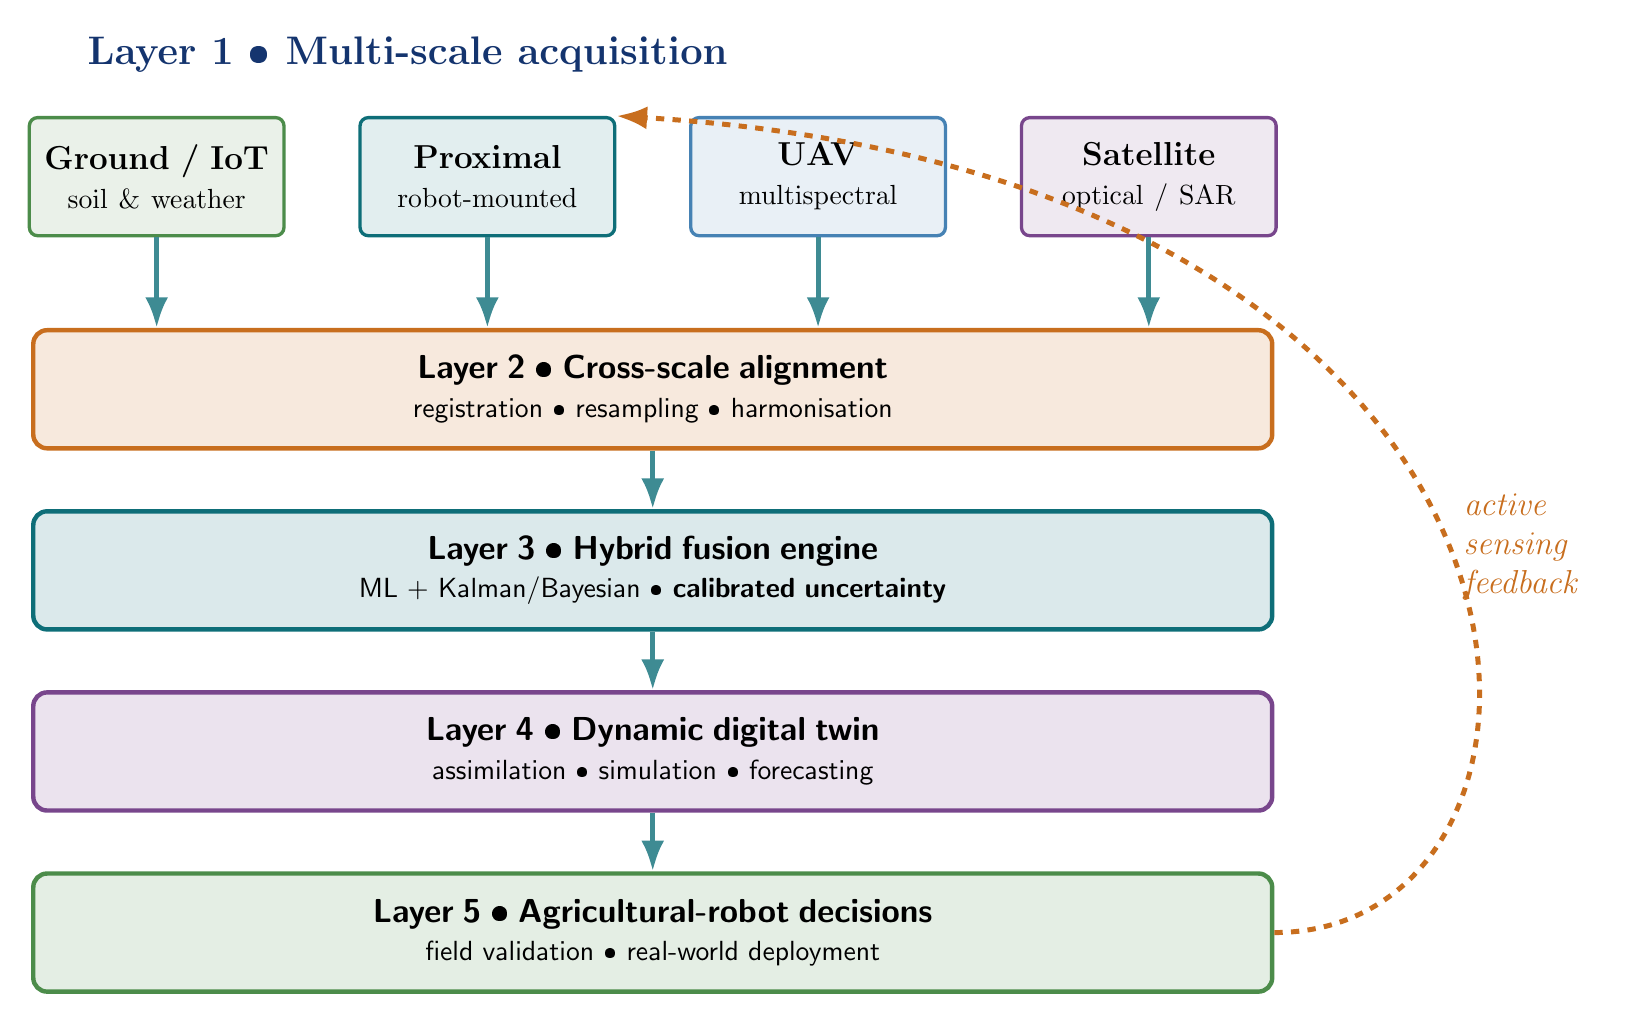
\begin{tikzpicture}[
  font=\sffamily,
  >=Latex,
  src/.style={rounded corners=3pt, draw=#1, line width=1.2pt, fill=#1!12,
              text width=3.0cm, align=center, minimum height=1.5cm, font=\large},
  layer/.style={rounded corners=5pt, draw=#1, line width=1.6pt, fill=#1!15,
                text width=15.5cm, align=center, minimum height=1.5cm},
  lbl/.style={font=\Large\bfseries, color=#1},
  sub/.style={font=\large, color=black!75},
  arr/.style={->, line width=1.8pt, color=accent!80},
]

% ---- Layer 1: four sources ----
\node[src=leaf]   (s1) at (0,0)    {\textbf{Ground / IoT}\\\normalsize soil \& weather};
\node[src=accent] (s2) at (4.2,0)  {\textbf{Proximal}\\\normalsize robot-mounted};
\node[src=sky]    (s3) at (8.4,0)  {\textbf{UAV}\\\normalsize multispectral};
\node[src=plum]   (s4) at (12.6,0) {\textbf{Satellite}\\\normalsize optical / SAR};
\node[lbl=navy, anchor=west] at (-1.0,1.55) {Layer 1 \textbullet\ Multi-scale acquisition};

% ---- Layer 2 ----
\node[layer=orange] (l2) at (6.3,-2.7)
   {\textbf{\large Layer 2 \textbullet\ Cross-scale alignment}\\[2pt]\sub registration \textbullet\ resampling \textbullet\ harmonisation};

% ---- Layer 3 ----
\node[layer=accent] (l3) at (6.3,-5.0)
   {\textbf{\large Layer 3 \textbullet\ Hybrid fusion engine}\\[2pt]\sub ML + Kalman/Bayesian \textbullet\ \textbf{calibrated uncertainty}};

% ---- Layer 4 ----
\node[layer=plum] (l4) at (6.3,-7.3)
   {\textbf{\large Layer 4 \textbullet\ Dynamic digital twin}\\[2pt]\sub assimilation \textbullet\ simulation \textbullet\ forecasting};

% ---- Layer 5 ----
\node[layer=leaf] (l5) at (6.3,-9.6)
   {\textbf{\large Layer 5 \textbullet\ Agricultural-robot decisions}\\[2pt]\sub field validation \textbullet\ real-world deployment};

% arrows sources -> L2
\draw[arr] (s1.south) -- (l2.north -| s1.south);
\draw[arr] (s2.south) -- (l2.north -| s2.south);
\draw[arr] (s3.south) -- (l2.north -| s3.south);
\draw[arr] (s4.south) -- (l2.north -| s4.south);
% L2->L3->L4->L5
\draw[arr] (l2) -- (l3);
\draw[arr] (l3) -- (l4);
\draw[arr] (l4) -- (l5);

% active-sensing feedback loop (right side, dashed orange)
\draw[->, line width=1.8pt, color=orange, dashed]
   (l5.east) .. controls (18.5,-9.6) and (18.5,0) .. (s2.north east)
   node[midway, right=2pt, font=\large\itshape, color=orange, align=left] {active\\sensing\\feedback};

\end{tikzpicture}
\end{document}
